\subsection{Your own image processing algorithm (Optional)}
\label{sect:prize}

In this task, you will perform an image manipulation of your choice.
The core of this transformation are three functions:
\begin{quote}
\begin{lstlisting}
int result_width(int width, int height)
int result_height(int width, int height)
pixel_t[] manipulate(pixel_t[] pixels, int width, int height)
\end{lstlisting}
\end{quote}
If \lstinline'I' is the representation of an image with width
\lstinline'w' and height \lstinline'h', then the result of calling
\lstinline'manipulate(I,w,h)' should the representation of image of
width \lstinline'result_width(w,h)' and height
\lstinline'result_height(w,h)'.

\begin{ectask}
\TAGS{array, safety}
  Create a C0 file \lstinline'manipulate.c0' implementing the three
  functions described above: \lstinline'result_width',
  \lstinline'result_height', and \lstinline'manipulate'. You may
  include any auxiliary functions you need in the same file, but you
  should not include a \lstinline'main()' function. You may not add
  arguments to \lstinline'manipulate', but you can write a separate
  function \lstinline'my_manipulate' (or whatever) and then call your
  function from the \lstinline'manipulate' function with some specific
  arguments.
\end{ectask}

You should look at \lstinline'README.txt' to see how to compile and run
this transformation against \lstinline'manipulate-main.c0'.

If you choose to do this task, be creative! Submissions will be
displayed on the Autolab scoreboard and we will highlight exemplary
submissions.
%To include your image in the scoreboard,
%use the \lstinline|handin| script and include the file \lstinline'output.png'
%-- if you don't include \lstinline'output.png', we'll use
%\texttt'g5.png'.
%
If you include a (small!) file \lstinline'manipulate.png',
we'll run your transformation against that image; otherwise
we'll run your transformation on \lstinline'g5.png'.

\begin{figure}[h]
\begin{center}
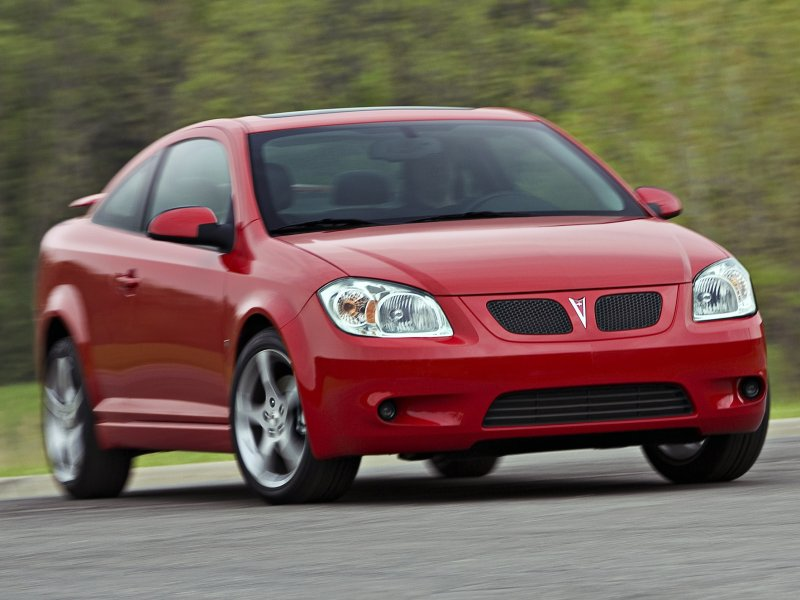
\includegraphics[scale=0.3]{\img/g5.png}
\end{center}
\caption{Manipulate me!}
\end{figure}


%%% Local Variables:
%%% mode: latex
%%% TeX-master: "main"
%%% End:
